\chapter{Instalace a nastavení SolidWorks}
\section{Instalace SolidWorks SDK}

\subsection*{Stažení instalátoru a získání licenčních klíčů}
Začneme otevřením webové stránky \href{http://www.solidworks.com/sdk}{www.solidworks.com/sdk}.
Zobrazí se nám formulář, do kterého vyplníme údaje o sobě (jméno, příjmení, e-mail a status - student).
Je nutné psát \B{bez diakritiky}!

\fxnote[author=PŠ]{\textcolor{mygreen}{Sem přijde screenshot formuláře}}

V sekci \B{Product information} pod textem \B{\enquote{I already have a Serial Number that starts with 9020}} zaškrtneme možnost \B{No} a do kolonky níže napíšeme \B{9SDK2019}.
Na pravé straně poté zaškrtneme nejnovější verzi, tedy \B{2020-2021}.
Vyplněný formulář odešleme kliknutím na tlačítko \B{Request download}.
Na další stránce potvrdíme licenční podmínky tlačítkem \B{Accept and Continue}.

Nyní jsme se již dostaly na stránku, odkud můžeme SDK stáhnout.
Klikneme tedy na tlačítko \B{Download}, čímž si stáhneme instalátor.
Okno ještě \B{nezavíráme} - budeme z něj potřebovat zkopírovat licenční čísla. 

\subsection*{Instalace}
Stažený instalátor otevřeme. 
Objeví se nám okno, ve kterém můžeme nastavit, kam chceme vyextrahovat soubory instalace.
Jakmile máme umístění zvolené, klikneme na tlačítko \B{Unzip}.
Chvíli počkáme a otevře se nám \It{Manažer instalací SOLIDWORKS 2020}.
Pokud se nám objeví okno informující, že po předchozí instalaci nebyl dokončen restart systému, stačí jej odklepnout tlačítkem \B{OK}.
Na obrazovce, kde můžeme zvolit typ instalace ponecháme zaškrtnuté \It{Instalovat na tento počítač} a klikneme na \B{Další}.

Nyní po nás bude instalátor chtít zadat sériová čísla. 
Otevřeme si tedy webový prohlížeč se stránkou, kde byla tato čísla napsaná.

\section{Instalace školních šablon a norm. dílů}

\subsection*{Stažení .ZIP archivu}
Nejprve je potřeba si stáhnout .ZIP soubor, který šablony a norm. díly obsahuje.
Nalezneme jej na adrese \href{https://bit.ly/CAD1921XE}{bit.ly/CAD1921XE}.
Stažený zip soubor si otevřeme a podle toho, jestli máme verzi SolidWorks 2019, nebo 2020 si na plochu zkopírujeme jednu ze dvou složek v něm obsažených (2019-2020 pro 2019, 2020-2021 pro 2020).

\subsection*{Instalace šablon a knihoven materiálů}
Zkopírovanou složku otevřeme.
Složku \It{Šablony SolidWorks...} si z ní přesunu na plochu a opět ji otevřu.
V novém okně průzkumníka Windows otevřeme disk C:, kam zkopírujeme obsah této složky (tedy složky \B{Program Files a ProgramData}).
Systém se zeptá, zda-li chceme některé soubory nahradit, vybereme že tak chceme učinit.
Původní složku \It{Šablony SolidWorks...} můžeme smazat, již ji nebudeme potřebovat.

\subsection*{Instalace normalizovaných dílů}
Na ploše máme stále složku s podsložkami \B{NORMALIZOVANÉ DÍLY, NORMALIZOVANÉ PRVKY, NORMALIZOVANÉ PROFILY a TECHNICKÉ KRESLENÍ}, přejmenujeme ji na lépe dohledatelný název, například \It{CAD\_SOKOLSKA}.
Přejmenovanou složku přesuneme do složky \B{Dokumenty}.

\noindent Nyní otevřeme SolidWorks.
Na pravé straně klikneme na kartu \It{Knihovna návrhů}.
Otevře se boční panel.
Na jeho horní straně je několik tlačítek, klikneme na \It{Přidat umístění souboru}.
V dialogovém okně otevřeme složku \It{Dokumenty} a v ní \It{CAD\_SOKOLSKA}.
Nyní klikneme na OK, čímž se nám složka přidá do knihovny návrhů.

\section{Zprovoznění RealView na necertifikovaném počítači}
\subsection*{Co je to režim RealView?}
Režim zobrazení RealView umožňuje věrnější zobrazení modelů díky vylepšenému stínování a odleskům.
Tento režim je ale podporován jen relativně malým počtem certifikovaných grafických karet NVIDIA Quadro a Radeon Pro.
Aktivace na ostatních grafických kartách je možná s malým zásahem do registru.\newline

\noindent\textcolor{red}{VAROVÁNÍ: Při aktivaci budeme zasahovat do registru systému, je tedy nutné se přesně řídit návodem. Zásah v registru na špatném místě může způsobit nestabilitu operačního systému, nebo aplikací.}

\subsection*{Zjištění označení aktuální grafické karty}
Než začneme cokoliv dělat, musíme zkontrolovat, že je SolidWorks vypnutý. 
Pokud ne, hned tak učiníme.
Na klávesnici zmáčkneme klávesovou zkratku \B{Win + R}, otevře se nám dialog \It{Spustit}.
Do políčka napíšeme \It{regedit} a potvrdíme Enterem.
Kliknutím na tlačítko \It{Ano} potvrdím udělení administrátorských oprávnění v okně \It{UAC}.

V levé části editoru registru postupně proklikáváme složky \newline HKEY\_CURRENT\_USER $>$ SOFTWARE $>$ SolidWorks $>$ SOLIDWORKS 2020 $>$ Performance $>$ Graphics $>$ Hardware $>$ Current.
Při kliknutí na poslední složku se nám vpravo objeví několik hodnot, klikneme dvakrát na \It{Renderer}.
Otevře se nám tabulka nastavení hodnoty, za pomoci \B{Ctrl + C} si její údaj celý zkopíruji (např. \It{GeForce GTX 1050/PCIe/SSE2}).

\subsection*{Přidání vlastního klíče do registru}
V levé straně editoru registru nyní otevřu složku \It{GI2Shaders}.
Následně si podle toho, jakou mám grafickou kartu vyberu složku \It{Other} (pokud mám graf. procesor Intel HD Graphics), nebo \It{NV40} (cokoliv ostatního) -- obě jsou obsaženy ve složce \It{GI2Shaders}.
Na zvolenou složku (Other, nebo NV40) kliknu pravým tlačítkem a vytvořím \It{nový klíč}, do jehož názvu vložím hodnotu, kterou jsem si před chvílí zkopíroval za pomoci \B{Ctrl + V}.
Zkontroluji, že je nový klíč vybraný a na pravé straně editoru registru kliknu opět pravým tl. myši.
Tentokrát vytvořím novou \It{Hodnotu DWORD (32 bitová)}, kterou nazvu \It{Workarounds}.
Na novou hodnotu dvakrát poklepu myší a do políčka \enquote{\It{Údaj hodnoty}} napíšu \B{4000080} pro verzi SolidWorks 2020.
Verze 2019 má tento kód lehce odlišný -- \B{30408}.

\subsection*{Vyzkoušení, zda nám RealView funguje}
Teď již jen musíme vyzkoušet, zda nám RealView funguje jak má.
Otevřeme SolidWorks a v něm nějaký díl, nebo sestavu.
Nahoře klikneme na tlačítko se symbolem oka a pokud se mezi možnostmi objeví i RealView, vše je v pořádku. 

\newpage

%%% Výkresovka - textové přepisy návodů
\chapter{Výkresová dokumentace - vybrané návody}
\fxnote[author=PŠ]{\textcolor{mygreen}{Sekci dopíšu, jakmile začnu točit videa z výkresovky}}

\section{Výkres hřídele}

\subsection{Hlavní a připojovací rozměry}

\subsection{Drážka pro pero}

\subsection{Drážka pro pojist. kroužek}

\newpage

%%% Vybrané text. návody z modelování
\chapter{Modelování - vybrané návody}

%%% Drážka pro pero v náboji
\section{Drážka pro pero v náboji}

\subsection*{Skica}
Vytvoříme kružnici na jedné ze základních ploch a zakótujeme ji průměrem hřídele, na který chceme náboj nasadit.
Na horní obvodový bod kružnice umístíme střed \It{obdélníku s počátkem ve středu}.

Šířka tohoto obdélníku je shodná s velikostí šířky drážky (hodnota \B{b} v ST).
Výška obdélníku musí být kótovaná vůči protilehlé hraně kružnice, kterou vybereme s podržením klávesy \It{SHIFT}.
Hodnotu kóty získáme součtem výšky \B{T\subscript{1}} a průměru hřídele/díry.

\subsection*{Odebrání vysunutím}
V nabídce \It{Prvky} vybereme prvek \It{Odebrání vysunutím}.
Vybereme všechny 3 oblasti, které ve skice vzniknou a hloubku nastavíme na \It{Skrz vše}.
Díra s drážkou pro pero je takto hotová.

%%% Drážka pro pero - hřídel
\section{Drážka pro pero na hřídeli}
\fxnote[author=PŠ]{\textcolor{mygreen}{Video ještě není hotové.}}

\subsection*{Vytvoření roviny}

\subsection*{Skica}

\subsection*{Odebrání vysunutím}

%%% Drážka pro PK - náboj
\section{Drážka pro pojist. kroužek v náboji}
\fxnote[author=PŠ]{\textcolor{mygreen}{Video ještě není hotové.}}

\subsection*{Skica}

\subsection*{Odebrání rotací}

%%% Drážka pro PK - hřídel
\section{Drážka pro pojistný kroužek na hřídeli}
\fxnote[author=PŠ]{\textcolor{mygreen}{Video ještě není hotové.}}

\subsection*{Skica}

\subsection*{Odebrání rotací}

%%% Čelní ozubené kolo s přímým ozubením - modelované splajnem
\section{Čelní ozubené kolo s přímým ozubením}

\subsection*{Vytvoření základního válce}

\subsection*{Profilová skica zubu}

\subsection*{Přidání vysunutím}

\subsection*{Zkosení a zaoblení}

%%% Řetězové kolo
\section{Řetězové kolo}

\subsection*{Vytvovření základního \enquote{talíře} pomocí přidání rotací}

\subsection*{Skica profilu drážek}

\subsection*{Odebrání vysunutím}

\newpage

%%% Vybrané text. návody z práce se sestavami
\chapter{Práce se sestavami - vybrané návody}

\section{Jak správně přejmenovat díl v sestavě?}
Občas se stane, že nazveme díl špatným názvem a následně jej chceme přejmenovat.
Každý, kdo to ale v SolidWorks někdy zkoušel ví, že to není tak úplně nejjednodušší záležitost.
V následujících pár řádcích se pokusím tuto problematiku objasnit.

\subsection*{Struktura projektů v SolidWorks}
Pro práci se sestavami je dobré vědět, jak fungují vazby a reference mezi soubory.
Tyto vazby přehledně ukazuje \autoref{fig:SOLIDWORKS_part-assembly-drawing}.
\begin{figure}[htpb]
    \centering
    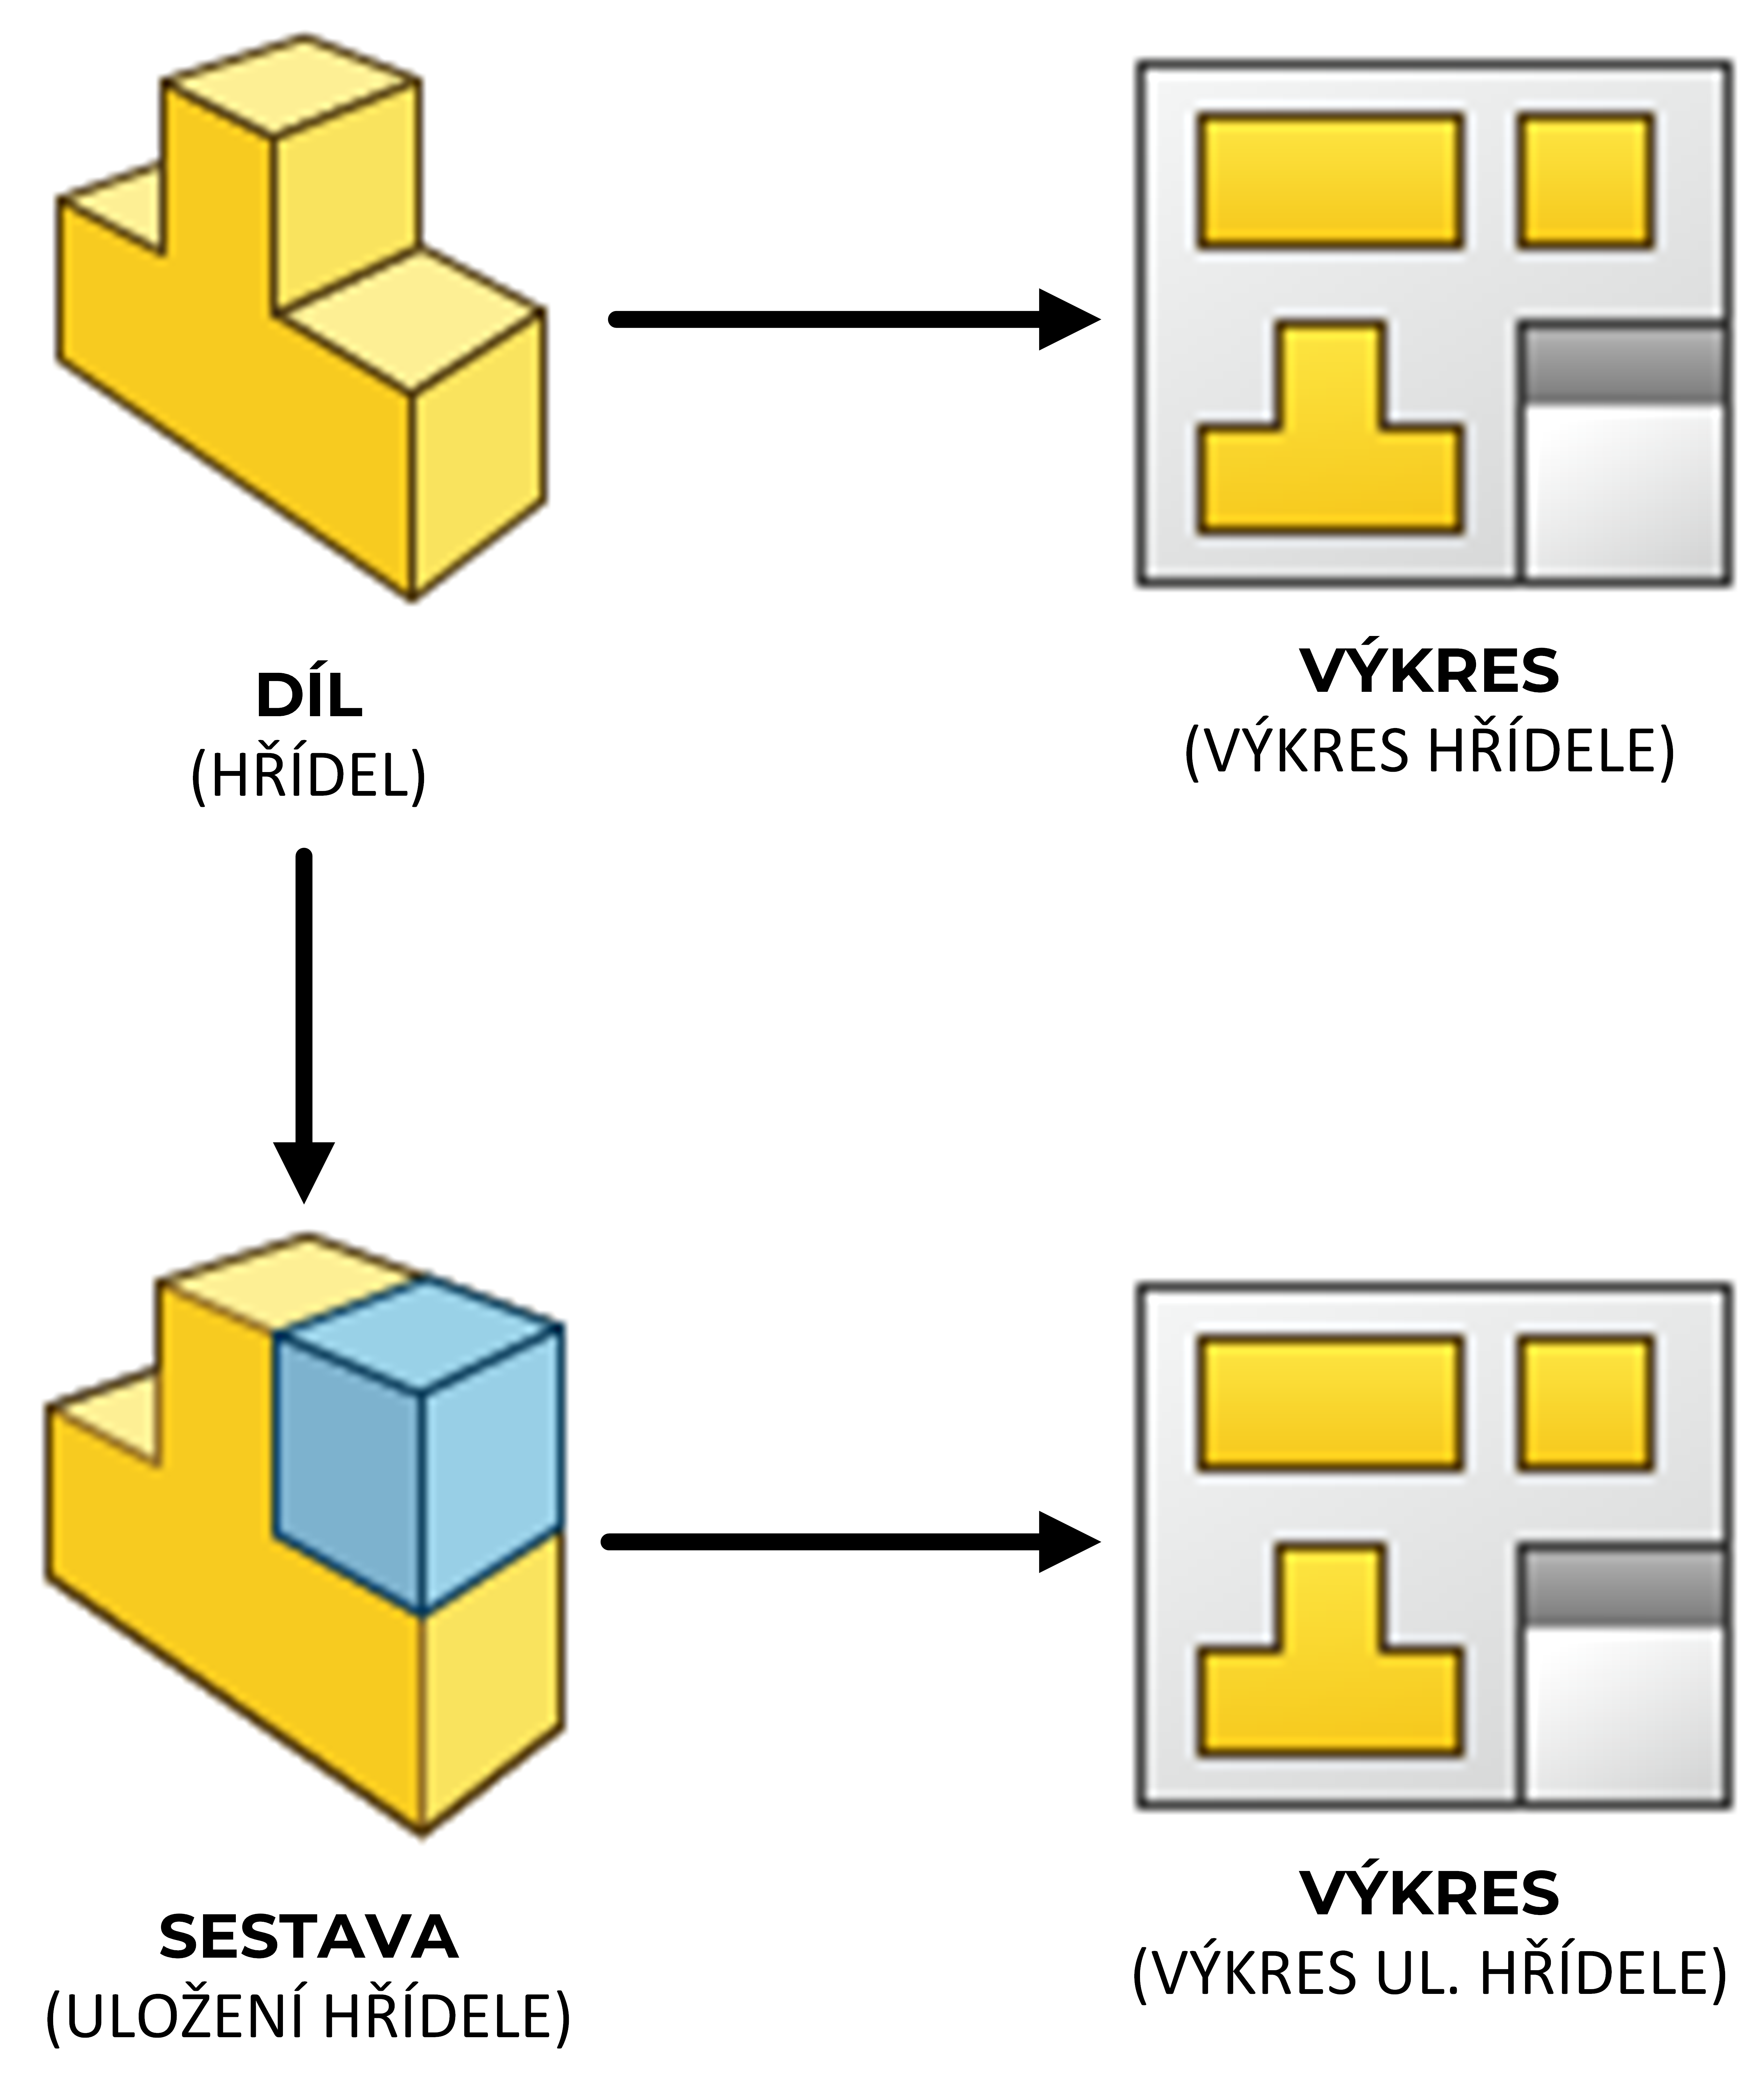
\includegraphics[width=0.35\textwidth]{img/graphics/png/SOLIDWORKS - PART-ASSEMBLY-DRAWING.png}
    \caption{Ilustrace vztahů mezi typy souborů SolidWorks}
    \label{fig:SOLIDWORKS_part-assembly-drawing}
\end{figure}

Pro to, abychom museli řešit přejmenovávání dílů v sestavách co nejméně, je dobré nazývat soubory správně již při vytváření.
Máme-li tedy nějaký díl (pro příklad vezměme ozubené kolo), pojmenujme jej tedy rovnou jako pastorek, nebo ozubené kolo.
Pokud již na začátku díl nazveme jako \enquote{kolečko}, \enquote{něco}, nebo zůstaneme u výchozího názvu \enquote{Díl1}, přijdeme později na to, že se v sestavě nedá orientovat, nebo že se v souborech nevyznáme.

\subsection*{Jak tedy na přejmenování dílu v sestavě?}
Prvoplánově může člověka napadnout si díl zobrazit v průzkumníkovi Windows, kliknout na něj pravým tl. myši a přejmenovat jej. 
Tím sice díl přejmenuje, ale všechny sestavy a výkresy, které na tento soubor před přejmenováním odkazovaly přestanou fungovat.

Správný postup je otevřít si sestavu, nebo výkres ve kterém se daný díl/sestava nachází a následně samotný díl, nebo sestavu, které chceme přejmenovat.
V nabídce \It{\enquote{Soubor}} u přejmenovávaného dílu/sestavy vybereme uložit jako a zvolíme první možnost - tedy uložení jako nový soubor s nahrazením vazeb.
Následně soubor uložíme s novým názvem, přepneme se na sestavu/výkres ve které je přejmenovaný díl obsažen, klikneme na tlačítko obnovit a na závěr sestavu/výkres uložíme.
Přejmenování je hotové a bez zbytečného rozbití vazeb.

\section{Jak správně přesunout sestavu na jiný počítač?}
S tímto problémem se setká každý strojař alespoň jednou.
Máte hotový projekt, tedy kompletní modely, výkresy, sestavu a chystáte se ji odevzdat.
Problém nastane ve chvílí, kdy 

\newpage